\subsection{Test Plan Verification}\label{sec:mtpVV}
The goal of Test Plan verification is to evaluate all test plan documents for
correctness, consistency, completeness, readability, feasibility, and
traceability.

\paragraph{Method} The test plan verification plan relies on peer
review/document inspection with the following stages:
\begin{enumerate}

    \item Preparation: Participants review the test plan documents with respect
    to their assigned role and goals (Table~\ref{tab:rolesTestPlan})

    \item Meeting: Participants meet to discuss findings, potential issues, and
    proposed action plans to address them

    \item Rework: The test plan author(s) revise the document(s) to address
    raised issues, guided by the proposed action plans

    \item Follow Up: Participants verify that raised issues have been addressed
    satisfactorily

\end{enumerate}

A recording device might be used to capture meeting proceedings in place of
physical note taking so that all participants can focus on the discussion.

Peer review/inspection begins when there is a new major version of a test plan
document. Peer review/inspection need be done on those documents only.

Peer review/inspection ends when reviewers agree that there are no issues that
will likely result in the inability to execute any element of the plans and
verify that all plan components contribute to \progname{}'s overall
verification and validation (V \& V).

\paragraph{Roles and Responsibilities} To assist in the achievement of their
assigned goals (Table~\ref{tab:rolesTestPlan}) using peer review/document
inspection:
\begin{itemize}

    \item Primary team members are responsible for ensuring that reviewers have
    the necessary materials, moderating the inspection process and reading
    through the test plan document(s) during the meeting

    \item Secondary and tertiary members are reviewers whom are responsible for
    reviewing the test plan document(s) prior to the meeting so that they are
    prepared to discuss it with the team

\end{itemize}

\paragraph{Inputs}
\begin{itemize}

    \item Concept Summary for \progname{}: A Computational Model of Emotion for
    Enhancing Non-Player Character Believability in Games

    \item Master Test Plan for \progname{}: A Computational Model of Emotion
    for Enhancing Non-Player Character Believability in Games

    \item Acceptance Test Plan for \progname{}: A Computational Model of
    Emotion for Enhancing Non-Player Character Believability in Games

    \item System, Integration, and Unit Test Plan for \progname{}: A
    Computational Model of Emotion for Enhancing Non-Player Character
    Believability in Games

    \item Review guide for \progname{}'s Master Test Plan (MTP)
    (Appendix~\ref{appendix:mtpInspection})

    \item Review guide for \progname{}'s Acceptance Test Plan (ATP)
    (Appendix~\ref{appendix:validationInspection})

    \item Review guide for \progname{}'s System, Integration, and Unit Test
    Plan (SIUTP) (Appendix~\ref{appendix:siutpInspection})

\end{itemize}

\paragraph{Outputs}
\begin{itemize}

    \item Objective evidence to assess the verification of the MTP, ATP, and
    SIUTP

    \item Objective evidence that the test plans are able to determine if their
    associated SDAs conform to their requirements and satisfy their testing
    criteria

    \item Objective evidence that the test plans are able to determine if
    \progname{} satisfies its allocated system requirements and its intended
    use and user needs

    \item Input to Master Test Report (MTR)

\end{itemize}

\paragraph{Estimated Completion Time} Five (5) weeks

Verification of test plan documentation is divided into parts. Only one part is
tested per week to reduce participant fatigue and to better coordinate with the
corresponding stage in the Software Development Life Cycle (SDLC):
\begin{itemize}

    \item Part 1: Master Test Plan

    \item Part 2: Acceptance Test Plan

    \item Part 3: System, Integration, and Unit Test Plan:
    Introduction/Preamble, System Test Plan

    \item Part 4: System, Integration, and Unit Test Plan: Integration Test Plan

    \item Part 5: System, Integration, and Unit Test Plan: Unit Test Plan

\end{itemize}

\begin{figure}[!h]
    \centering
    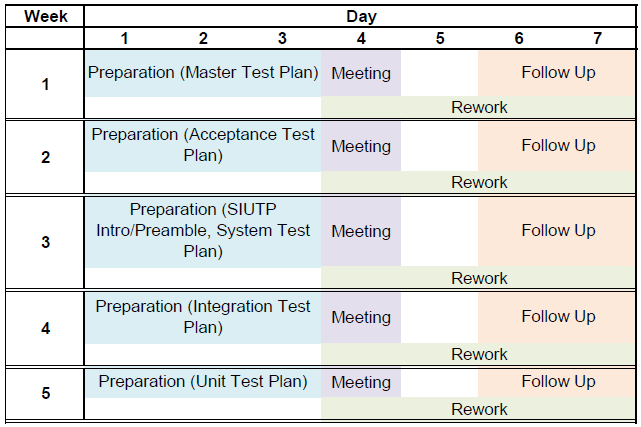
\includegraphics[width=0.8\linewidth]{figures/TP_Schedule.png}
\end{figure}